\documentclass[12pt,letterpaper]{article}

\usepackage{fancyhdr}
\pagestyle{fancy}
\fancyhf{}
\rhead{Vaja 8}
\lhead{ORS}
\setlength{\headheight}{16pt}

\usepackage[utf8]{inputenc}
\usepackage[slovene]{babel}
\usepackage[colorlinks = true, urlcolor = blue]{hyperref}

\usepackage{xcolor}
\usepackage{listings}
\usepackage{graphicx}
\graphicspath{{./images/}}
\definecolor{mGreen}{rgb}{0,0.6,0}
\definecolor{mGray}{rgb}{0.5,0.5,0.5}
\definecolor{mPurple}{rgb}{0.58,0,0.82}
\definecolor{backgroundColour}{rgb}{1,1,1}

\lstdefinestyle{CStyle}{
    backgroundcolor=\color{backgroundColour},
    commentstyle=\color{mGreen},
    keywordstyle=\color{magenta},
    numberstyle=\tiny\color{mGray},
    stringstyle=\color{mPurple},
    basicstyle=\footnotesize,
    breakatwhitespace=false,
    breaklines=true,
    captionpos=b,
    keepspaces=true,
    numbers=left,
    numbersep=5pt,
    showspaces=false,
    showstringspaces=false,
    showtabs=false,
    tabsize=2,
    language=C,
    frame=none
}

\begin{document}

\begin{center}
    \textbf{\Large Komunikacija z UART v STM32F4}
\end{center}

Na tokratni vaji se bomo spoznali še z enim tipom naprave za serijsko komunikacijo. Imenuje se Universal Asynchronous Receiver/Transmitter oziroma krajše UART. UART je torej naprava, ki omogoča asinhrono serijsko komunikacijo. Obstajajo tudi naprave, ki ponujajo poleg asinhrone tudi sinhrono komunikacijo, le-te označujemo s kratico USART. USART torej označuje naprave, ki omogočajo tako sinhron kot asinhron prenos. Na tokratni vaji se bomo posvetili predvsem asinhroni različici.

Mikrokrmilniške USART naprave običajno delujejo s signali z napetostmi od 0V do 3,3V ali 5V. Obstajajo pa tudi dodatni moduli, ki omogočajo da USART signale pošiljamo v skladu s standardom RS-232. Slednji je telekomunikacijski standard, ki določa, da je logična enica predstavljena z napetostjo od -25V do -3V, logična ničla pa z napetostjo od 3V do 25V. Klasični računalniški serijski porti, ki jih danes sicer poredko srečamo v osebnih računalnikih in prenosnikih, delujejo na napetostnih nivojih od -13V do 13V. Včasih so bili serijski porti standardni del vsakega računalnika, saj so služili za komunikacijo z dial-up modemi, čitalci za črtne kode, CNC stroji, igralnimi palicami (angl. joystick) ter množico ostalih naprav.

Danes se USART standard samostojno ali v navezavi s standardi RS-232 uporablja za komunikacijo med mikrokrmilniki, z GPS senzorji, moduli za Bluetooth, WiFi, Ethernet, Zigbee in podobno. Pogosto jih srečujemo tudi v industrijskih aplikacijah. Praktično ni mikrokrmilniškega sistema, ki ne bi uporabljal UART naprav.


\section*{Povezava UART naprav}

Najenostavnejši in hkrati najpogostejši priklop dveh UART naprav je prikazan na sliki \ref{simpleuart}. Na napravah uporabimo zgolj pina TX (Transmit) in RX (Receive) ter GND. Pin TX je namenjen pošiljanju, RX pa sprejemanju, zato jih povežemo križno. Povežemo tudi GND pin, da zagotovimo usklajenost logičnih nivojev na obeh straneh.

\begin{figure}[ht!]
  \centering
  \caption{Enostavna vezava UART naprav.}
  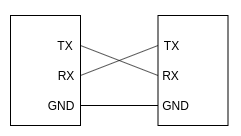
\includegraphics[width=180pt]{images/vaja8/uart_simple.png}
  \label{simpleuart}
\end{figure}

\subsection*{UART HFC (Hardware Flow Control)}

Dodatno lahko na napravah uporabimo še pina CTS (Clear to Send) in RTS (Request to Send). Omenjena pina sta namenjena temu, da se UART napravi uskladita kdaj sta pripravljeni za sprejem podatkov. Če je naprava pripravljena na sprejem podatkov, pin RTS postavi na nizko logično vrednost. Na pinu CTS pa naprava preveri, če je naprava na drugi strani pripravljena za sprejem. Ko oba pina na povezanih napravah povežemo križno, kot je prikazano na sliki \ref{uartctsrts}, dobimo povezani napravi, ki pošiljata zgolj, ko je naprava na drugi strani pripravljena. Preverjanje in nastavljanje RTS in CTS pinov se v UART napravi izvaja strojno, brez programskega posredovanja.

HFC se uporablja predvsem pri visokih prenosnih hitrostih, ko prenašamo velike količine podatkov ali ko je naprava, ki sprejema podatke počasna.

\begin{figure}[ht!]
  \centering
  \caption{Enostavna vezava UART naprav z uporabo Hardware Flow Control signalov.}
  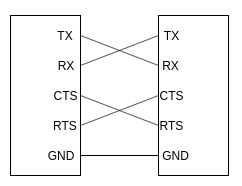
\includegraphics[width=180pt]{images/vaja8/uart_cts_rts.png}
  \label{uartctsrts}
\end{figure}


\section*{Asinhron prenos}

V mirujočem stanju mora biti prenosna linija v visokem logičnem stanju (logična enica), kar se običajno zagotovi s pull-up uporom. Pojavitev ničle, ko je linija v mirujočem stanju, označuje začetek prenosa. Omenjena ničla se zato imenuje start bit. Start bitu sledi 8 ali 9 podatkovnih bitov. Podatkovnim bitom nato lahko sledi paritetni bit temu pa stop bit. V primeru, da paritetnega bita ne potrebujemo stop bit sledi takoj za podatkovnimi biti. Primer prenosa števila 0x61 (0110 0001) brez paritetnega bita je prikazana na sliki \ref{asinhronprenos}.

\begin{figure}[ht!]
  \centering
  \caption{Primer prenosa števila 0x61 (0110 0001).}
  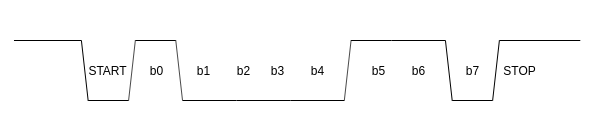
\includegraphics[width=320pt]{images/vaja8/asinhron_prenos.png}
  \label{asinhronprenos}
\end{figure}

Hitrost prenosa je pri UART napravah podana v baudrate-u, kar označuje število simbolov na sekundo. Tipične vrednosti za baudrate so 9600, 19200, 38400, 57600, 115200, 230400, 460800 in 921600. UART napravi, ki nastopata v prenosu, morata imeti usklajen baudrate. V nasprotnem primeru prenos ne bo uspešen. Prav tako morata napravi biti usklajeni v pariteti ter dolžini stop bit periode. Ta je lahko enaka času prenosa enega ali dveh bitov.


\section*{UART v STM32F4}

Krmilnik STM32F407, ki ga uporabljamo na vajah, ima 6 UART naprav: USART1, USART2, USART3, UART4 in UART5 ter USART6. Naprave 1,2,4 in 6 so torej sposobne asinhronega in sinhronega prenosa, napravi 4 in 5 pa zgolj asinhronega.

\subsection*{Inicializacija UART naprave}

Kot običajno moramo na začetku najprej prižgati uro U(S)ART naprave. To storimo z ukazom \texttt{\_\_HAL\_RCC\_USARTx\_CLK\_ENABLE()}, kjer \texttt{USARTx} predstalvlja oznako določene USART naprave. Bodite pozorni na razlike v imenih naprav (USART ali UART).

Nato je potrebno napravi določiti vse nastavitve prenosa. Te določimo s strukturo \texttt{UART\_HandleTypeDef}. Prvi element te strukture je, podobno kot pri inicializaciji SPI naprave, element \texttt{Instance} s katerim določite napravo, ki jo želite uporabljati. 

Drugi element strukture je struktura \texttt{Init}, ki hrani vse nastavitve UART prenosa. Posamezni elementi te strukture so opisani v nadaljevanju. Ko določimo vse nastavitve prenosa inicializiramo napravo s klicem funkcije \texttt{HAL\_UART\_Init(UART\_HandleTypeDef*)}.

\subsubsection*{Mode}

Nastavitev \texttt{Mode} določa namen za katerega bomo uporabili napravo. UART napravo namreč lahko uporabimo samo za sprejemanje (\texttt{UART\_MODE\_RX}), samo za pošiljanje (\texttt{UART\_MODE\_TX}) ali za oboje hkrati (\texttt{UART\_MODE\_TX\_RX}).

\subsubsection*{BaudRate}

Nastavitev \texttt{BaudRate} določa hitrost prenosa. Kot že rečeno, se največkrat uporablja vrednosti 9600, 19200, 38400, 57600, 115200, 230400, 460800 in 921600.

\subsubsection*{WordLength}

Z nastavitvijo \texttt{WordLength} določate koliko podatkovnih bitov se prenese v enemu UART prenosu. Možnosti sta 8 (\texttt{UART\_WORDLENGTH\_8B}) ali 9 bitov (\texttt{UART\_WORDLENGTH\_9B}).

\subsubsection*{Parity}

\texttt{Parity} določa želeno pariteto, ki je lahko liha (\texttt{UART\_PARITY\_ODD}), soda (\texttt{UART\_PARITY\_EVEN}) ali pa je ne uporabljamo ((\texttt{UART\_PARITY\_NONE}).

\subsubsection*{StopBits}

Lahko imamo en stop bit (\texttt{UART\_STOPBITS\_1}) ali dva (\texttt{UART\_STOPBITS\_2}).

\subsubsection*{HwFlowCtl}

\texttt{HwFlowCtl} nastavlja HFC, imamo več opcij:

\begin{itemize}
    \item \texttt{UART\_HWCONTROL\_NONE} -- HFC je izklopljen.
    \item \texttt{UART\_HWCONTROL\_RTS} -- uporabimo zgolj RTS.
    \item \texttt{UART\_HWCONTROL\_CTS} -- uporabimo zgolj CTS.
    \item \texttt{UART\_HWCONTROL\_RTS\_CTS} -- HFC uporabimo v celoti.
\end{itemize}

\subsubsection*{Primer inicalizacije}

Primer inicalizacije SPI naprave je prikazan spodaj, nastavljamo napravo USART1.

\begin{center}
\begin{lstlisting}[style=CStyle]
UART_HandleTypeDef uart;
uart.Instance = USART1;
uart.Init.BaudRate = 115200;
uart.Init.WordLength = UART_WORDLENGTH_8B;
uart.Init.StopBits = UART_STOPBITS_2;
uart.Init.Parity = UART_PARITY_ODD;
uart.Init.Mode = UART_MODE_TX;
uart.Init.HwFlowCtl = UART_HWCONTROL_RTS_CTS;
HAL_UART_Init(&uart);
\end{lstlisting}
\end{center}

\subsection*{Inicializacija GPIO pinov}

Poleg inicializacije UART naprave moramo, podobno kot pri časovnikih in SPI, inicializirati tudi pine, ki jih naprave uporabljajo. Nastavimo jih kot alternativne funkcije s push-pull (PP) brez pull-up ali pull-down uporov. V spodnji tabeli je prikazan seznam vezav pinov RX in TX za vseh 6 UART naprav v krmilniku STM32F407. Na sliki \ref{alternativne_funkcije} je zopet prikazan diagam vezav alternativne funkcije posameznih UART naprav.

\begin{table}[ht!]
    \small
    \caption{Vezava pinov UART naprav na GPIO pine.}
    \begin{center}
        \begin{tabular}{c|c|c|c|c|c|c}
            \textbf{Pin} & \textbf{USART1} & \textbf{USART2} & \textbf{USART3} & \textbf{UART4} & \textbf{UART5} & \textbf{USART6} \\ \hline
            RX & PB7 & PA3 & PB11 & PC11 & PD2 & PC7 \\ \hline
            TX & PB6 & PA2 & PB10 & PC10 & PC12 & PC6 \\
        \end{tabular}
    \end{center}
    \label{UARTPinsTable}
\end{table}

\begin{figure}[ht!]
  \centering
  \caption{Mapiranje alternativnih funkcij.}
  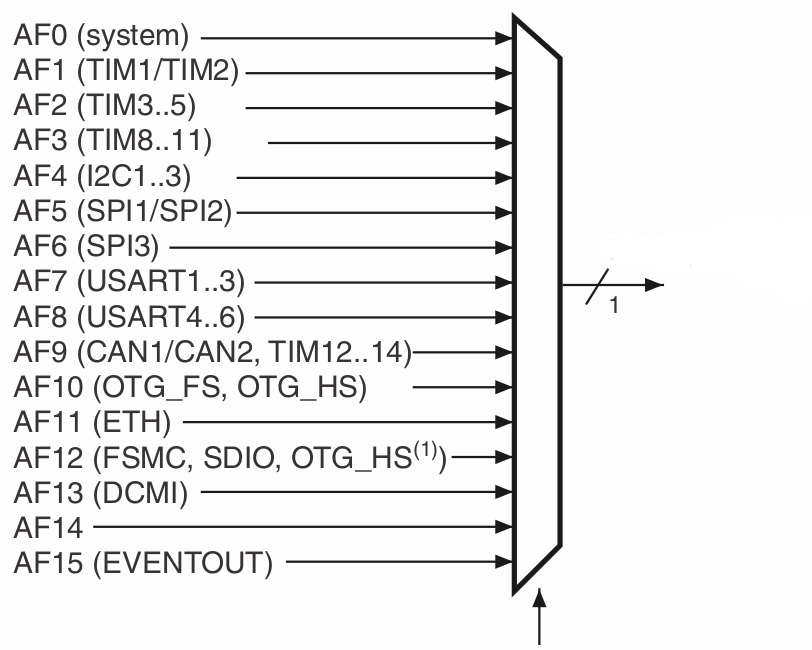
\includegraphics{images/vaja5/SPI_AF.png}
  \label{alternativne_funkcije}
\end{figure}

\subsection*{Pošiljanje in sprejemanje}

Funkcije za pošiljanje in sprejemanje so podobne tistim, ki smo jih uporabili pri SPI napravah. Za pošiljanje uporabimo funkcijo \texttt{HAL\_UART\_Transmit()}. Prvi parameter je kazalec na inicializacijsko strukturo UART naprave. Sledi kazalec na spremenljivko za pošiljanje. Z zadnjima dvema parametroma določimo število bajtov v prenosu ter maksimalni čas prenosa (angl. timeout) v milisekundah. V primeru, da je prenos zaključen znotraj maksimalnega dovoljenega časa, funkcija vrne \texttt{HAL\_OK}, v nasprotnem primeru pa \texttt{HAL\_TIMEOUT}. Primer uporabe omenjene funkcije je prikazan spodaj. Funkcija za sprejemanje \texttt{HAL\_UART\_Receive} je podobna funkciji za pošiljanje, s to razliko da podamo kazalec na spremenljivko kamor naj se shranijo podatki. Obe funkciji sta blokirajoči, kar pomeni, da lahko program nadaljuje šele, ko je pošiljanje ali sprejemanje zaključeno. To pa je pogosto neželjeno obnašanje, zato bomo v nadaljevanju spoznali tudi neblokirajoče klice, ki se izvajajo s pomočjo prekinitev.

\begin{center}
\begin{lstlisting}[style=CStyle]
uint8_t buffer[4]; 
// ali uint8_t buffer[] = "test";
HAL_UART_Receive(&uart, buffer, sizeof(buffer), HAL_MAX_DELAY);
HAL_UART_Transmit(&uart, buffer, sizeof(buffer), HAL_MAX_DELAY);
\end{lstlisting}
\end{center}

\subsection*{Zastavice}

Podobno kot pri napravi SPI tudi tu lahko spremljamo stanje naprave UART preko zastavic. Spodaj je zapisan seznam vseh pomembnejših zastavic s kratkimi opisi njihovega pomena. Stanje zastavice preverjamo s funkcijo \texttt{\_\_HAL\_UART\_GET\_FLAG()}, brišemo pa jih s funkcijo \texttt{\_\_HAL\_UART\_CLEAR\_FLAG()}. Zastavica RXNE (prejeli smo nove podatke) se pobriše samodejno, ko preberemo prispeli podatek, tako da nam te zastavice ni potrebno brisati programsko.

\begin{center}
\begin{lstlisting}[style=CStyle]
// uporabljen pri HW Flow Control. oznacuje da naprava lahko poslje podatek
UART_FLAG_CTS 
// lahko zacnemo naslednji prenos, funkcija Transmit zastavico preveri sama
UART_FLAG_TXE 
// zadnji prenos se je zakljucil
UART_FLAG_TC
// prejeli smo nov podatke
UART_FLAG_RXNE
// napaka paritete
UART_FLAG_PE
\end{lstlisting}
\end{center}

\subsection*{Prekinitve UART naprav}

Vse zastavice lahko uporabimo tudi za proženje prekinitev. Imena prekinitev se ujemajo z imeni zastavic, le da \texttt{\_FLAG\_} zamenjamo z \texttt{\_IT\_}. Za vklop prekinitve uporabimo funkcijo \texttt{\_\_HAL\_UART\_ENABLE\_IT()}, podobno kot ste to storili pri časovnikih. Ne pozabite, da je še vedno potrebno vklopiti prekinitve za izbrano UART napravo na prekinitvenem krmilniku (NVIC) ter jim določiti prioriteto. Spodaj je podana tabela prekinitvenih oznak ter imen prekinitveno-servisnih programov za vse UART naprave. V primeru realizacije branja s prekinitvami lahko znotraj PSP-ja uporabite funkcijo \texttt{HAL\_UART\_Receive}, le da v tem primeru vedno preberete samo en podatek (tisti, ki je bil ravnokar prejet), timeout pa obvezno nastavite na 0! V naslednjem podpoglavju bomo sicer spoznali bolj čisto rešitev za pošiljanje in branje s prekinitvami.


\begin{table}[ht!]
\centering
\begin{tabular}{c|c|c}
UART                         & Prekinitvene oznake               & Imena PSP-jev                           \\ \hline
\multicolumn{1}{c|}{USART1} & \multicolumn{1}{c|}{USART1\_IRQn} & \multicolumn{1}{c}{USART1\_IRQHandler} \\ \hline
\multicolumn{1}{c|}{USART2} & \multicolumn{1}{c|}{USART2\_IRQn} & \multicolumn{1}{c}{USART2\_IRQHandler} \\ \hline
\multicolumn{1}{c|}{USART3} & \multicolumn{1}{c|}{USART3\_IRQn} & \multicolumn{1}{c}{USART3\_IRQHandler} \\ \hline
\multicolumn{1}{c|}{UART4}  & \multicolumn{1}{c|}{UART4\_IRQn}  & \multicolumn{1}{c}{UART4\_IRQHandler}  \\ \hline
\multicolumn{1}{c|}{UART5}  & \multicolumn{1}{c|}{UART5\_IRQn}  & \multicolumn{1}{c}{UART5\_IRQHandler}  \\ \hline
\multicolumn{1}{c|}{USART6} & \multicolumn{1}{c|}{USART6\_IRQn} & \multicolumn{1}{c}{USART6\_IRQHandler}
\end{tabular}
\end{table}


\subsection*{Ne-blokirajoče pošiljanje in sprejemanje}

Poleg blokirajočih funkcij \texttt{HAL\_UART\_Transmit()} in \texttt{HAL\_UART\_Receive()} obstajata še funkciji, ki omogočata, da program nadaljuje z izvajanjem, branje in pošiljanje pa se spremlja in izvaja preko prekinitev. Za ta namen sta na voljo funkciji \texttt{HAL\_UART\_Transmit\_IT()} ter \texttt{HAL\_UART\_Receive\_IT()}. Omenjeni funkciji vklopita vse potrebne prekinitve USART naprave, ki se ob zaključku prenosa tudi izklopijo. 

Pri uporabi ne-blokirajočih UART funkcij je potrebno v PSP dodati še funkcijo  \texttt{HAL\_UART\_IRQHandler(UART\_HandleTypeDef*)}. Ta funkcija namesto vas poskrbi, da se v primeru sprejemanja, prebere prejeti podatek in shrani na pravilno mesto v podani spremenljivki. Funkcija v PSP-ju prav tako pobriše vse zastavice in v primeru, da so bili prejeti vsi pričakovani bajti izklopi prekinitve. V primeru pošiljanja funkcija v PSP-ju poskrbi, da se začne pošiljati naslednji želeni znak, oziroma zaključi pošiljanje, če so bili prenešeni vsi podatki. Prekinitveno servisni program za napravo USART2 morajo torej izgledati kot je prikazano spodaj.

\begin{center}
\begin{lstlisting}[style=CStyle]
void USART2_IRQHandler()
{
    HAL_UART_IRQHandler(&uart);
}
\end{lstlisting}
\end{center}

Če želimo, lahko ob zaključku pošiljanja \texttt{HAL\_UART\_IRQHandler()} pokliče tudi tako imenovano callback funkcijo. V primeru končanega po\-ši\-lja\-nja se pokliče funkcija \texttt{HAL\_UART\_TxCpltCallback(UART\_HandleTypeDef*)}, v primeru branja pa \texttt{HAL\_UART\_RxCpltCallback(UART\_HandleTypeDef*)}. Ti dve funkciji lahko definirate v poljubnem delu projekta. Bodite pa pozorni na to, da se funkciji kličeta iz prekinitveno-servisnega programa. To pomeni, da si tudi tu želimo, da se zaključita čimprej.
\newpage
\subsection*{Priprava projekta}

Za to, da lahko uporabimo UART funkcije moramo v projekt v STM32Cube dodati datoteke iz STM32 HAL knjižnice. Vse datoteke knjižnice se nahajajo na:

\begin{itemize}
    \item Windows:
    
    \texttt{C:/Users/<username>/Repository/STM32Cube\_FW\_F4\_V1.24.1\\/Drivers/STM32F4xx\_HAL\_Driver}
    
    \item Unix:
    
    \texttt{/home/username/STM32Cube/}
\end{itemize}

Za uporabo UART funkcij kopirajte \texttt{Src/stm32f4xx\_hal\_uart.c} iz knji\-žni\-ce v projekt na lokacijo \texttt{Drivers/STM32F4xx\_HAL\_Driver/Src}.

Nato skopirajte še datoteko \texttt{Inc/stm32f4xx\_hal\_uart.h} iz knjižnice v projekt na lokacijo \texttt{Drivers/STM32F4xx\_HAL\_Driver/Inc}.

Ko dodate datoteki, v \texttt{Inc/stm32f4xx\_hal\_conf.h} odkomentirajte vrstico, ki definira \texttt{HAL\_UART\_MODULE\_ENABLED}. Obe datoteki lahko najdete tudi na spletni učilnici, pri gradivu za vajo 8.

\newpage

\section*{Naloga}

Izberite poljubno UART napravo s katero realizirajte pošiljanje in sprejemanje dveh bajtov v kosu. Pošiljali in sprejemali boste ASCII nize (``ukaze'') s katerimi bomo krmilili LED diode. Ukaz Sx bo led diodo x prižgal, ukaz Rx pa jo bo ugasnil. Tako dobimo 8 pravilnih ukazov: S1, R1, S2, R2, S3, R3, S4 ter R4. Na primer ukaz S1 sporoči napravi, ki sprejema podatke, naj prižge prvo LED diodo, ukaz R1 pa sporoči, da želimo isto diodo ugasniti.

Komunikacija naj poteka z baudrate 115200, brez paritete in s stop bitom dolžine 1, HFC naj bo izklopljen. Sprejemni del mora biti sposoben sprejeti omenjene ukaze ter jih sprocesirati. Lahko predpostavite, da boste vedno prejeli pravilne ukaze, na primer ukaza K3 in S6 nista pravilna. Na strani pošiljanja implementirajte, da UART pošilja ponavljajoče zaporedje ukazov. Na primer:

\begin{itemize}
    \item pošlji S1,
    \item počakaj pol sekunde,
    \item pošlji S2,
    \item počakaj pol sekunde,
    \item pošlji R1,
    \item počakaj pol sekunde,
    \item pošlji R2,
    \item počakaj pol sekunde in ponovi.
\end{itemize}

\end{document}
